\section{Prérequis}
Pour la suite de ce document, l'ensemble du projet a été réalisé avec un environnement virtuel (conda).

\subsection{Vérification de la présence d'un GPU et installation de CUDA}

Pour profiter de l'accélération matérielle (ce qu'on vous recommande fortement) lors de l'entraînement de modèles, il est important de vérifier si votre ordinateur dispose d'un GPU compatible.

\begin{itemize}
    \item \textbf{Sous Windows :} Ouvrez le gestionnaire de tâches (\texttt{Ctrl+Shift+Esc}) et vérifiez l'onglet ``Performances'' pour voir si un GPU nvidia est détecté.
    \begin{verbatim}
    lspci | grep -i nvidia
    \end{verbatim}
\end{itemize}

\textbf{Installation de CUDA :}

\begin{enumerate}
    \item Rendez-vous sur le site officiel de NVIDIA : \url{https://developer.nvidia.com/cuda-downloads}. Pour l'Installer typeprenez la version local
    \item Sélectionnez votre système d'exploitation et suivez les instructions d'installation.
    \item Après installation, vérifiez la version de CUDA avec la commande :
    \begin{verbatim} 
                        nvcc --version
    \end{verbatim}
\end{enumerate}

\textbf{Remarque :} Assurez-vous que la version de CUDA installée est compatible avec la version de PyTorch que vous souhaitez utiliser (voir la documentation officielle de PyTorch).

\subsection{Installation de Pytorch}
Avant de commencer, munissez vous d'un environnement virtuel et assurez-vous d'avoir installé les dépendances nécessaires. L'ensemble des dépendances se retrouvent dans un fichier \texttt{requirements.txt} et sont facilement installables via \texttt{pip} ou \texttt{conda}.
Activez votre environnement virtuel et vous pourrez commencez à utiliser les commandes \texttt{bash} du guide utilisateur sur votre terminal.
Par ailleurs, une dépendance importante à prendre en compte est la library avec laquelle sont écrit les réseaux de neuronnes profonds : \textbf{\href{https://pytorch.org/get-started/locally/}{Pytorch}}.

\begin{figure}[H]
    \centering
    \href{https://pytorch.org/get-started/locally/}{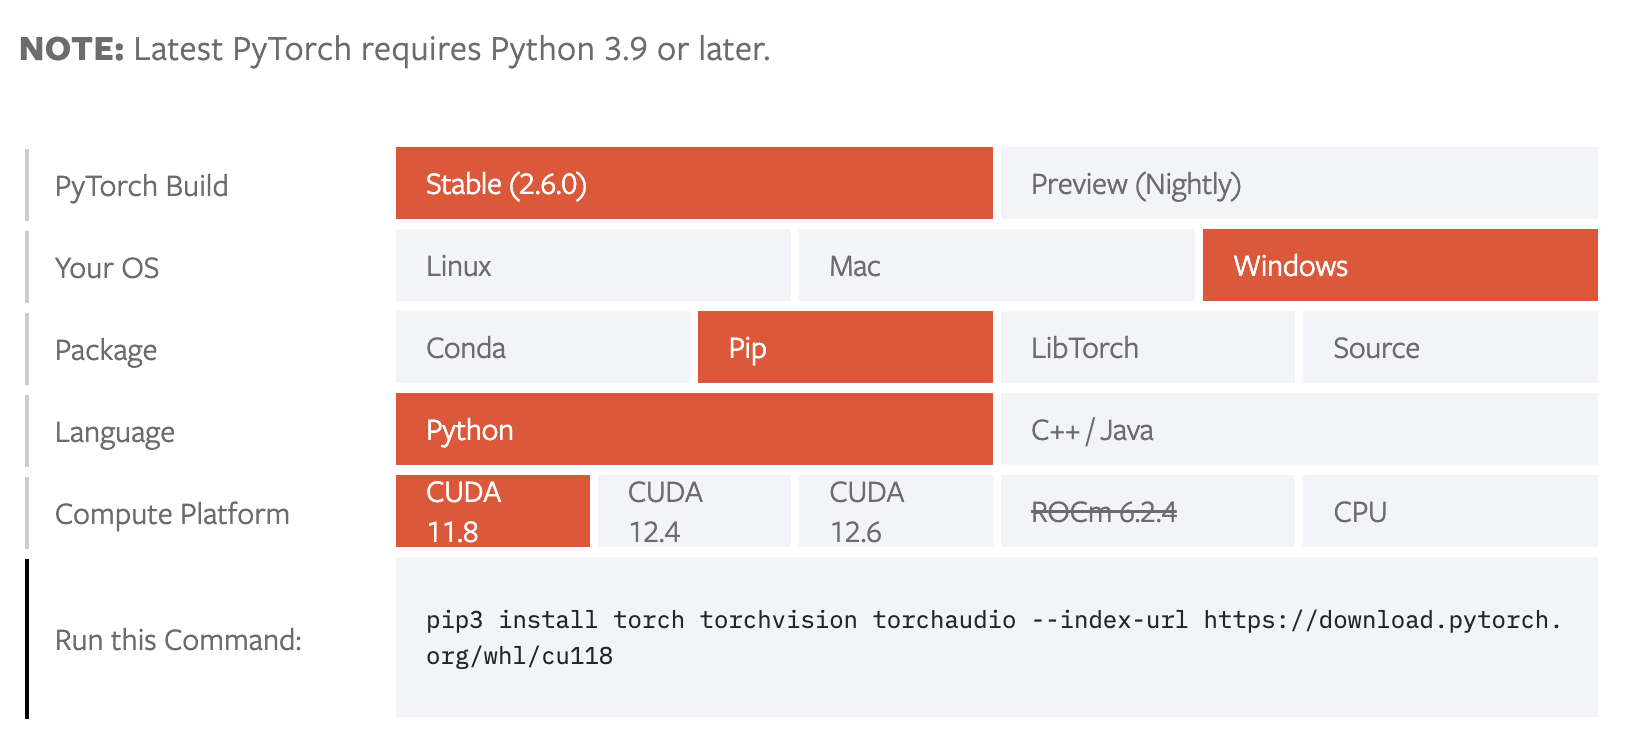
\includegraphics[width=0.6\textwidth]{GuideUtilisateur/pytorch.png}}
    \caption{Page de téléchargement de Pytorch}
\end{figure}

Pour vérifier la disponibilité du GPU avec \texttt{PyTorch}, lancez dans un terminal Python :
\begin{verbatim}
import torch
print(torch.cuda.is_available())
\end{verbatim}
Si la commande retourne \texttt{True}, votre GPU est prêt à être utilisé.